\documentclass[10pt,executivepaper]{article}
\usepackage[utf8]{inputenc}
\usepackage[spanish]{babel}
\usepackage{amsmath}
\usepackage{amsfonts}
\usepackage{amssymb}
\usepackage{graphics}
\usepackage{graphicx}
\usepackage[left=2cm,right=2cm,top=2cm,bottom=2cm]{geometry}
\usepackage{imakeidx}
\makeindex[columns=3, title=Alphabetical Index, intoc]
\usepackage{listings}
\usepackage{xcolor}
\usepackage{multicol}
\usepackage{changepage}
\usepackage{float}
\usepackage{cite}
\usepackage{url}
\usepackage{lscape}

\definecolor{codegreen}{rgb}{0,0.6,0}
\definecolor{codegray}{rgb}{0.5,0.5,0.5}
\definecolor{codepurple}{rgb}{0.58,0,0.82}
\definecolor{backcolour}{rgb}{0.95,0.95,0.92}

\lstdefinestyle{mystyle}{
    backgroundcolor=\color{backcolour},
    commentstyle=\color{codegreen},
    keywordstyle=\color{magenta},
    numberstyle=\tiny\color{codegray},
    stringstyle=\color{codepurple},
    basicstyle=\ttfamily\footnotesize,
    breakatwhitespace=false,
    breaklines=true,
    captionpos=b,
    keepspaces=true,
    numbers=left,
    numbersep=5pt,
    showspaces=false,
    showstringspaces=false,
    showtabs=false,
    tabsize=3
}

\lstset{style=mystyle}

\title{Actividad: Cálculo distribuido de PI}

\author{Instituto Politécnico Nacional\\Escuela Superior de Computo\\Desarrollo de Sistemas Distribuidos\\Adrian González Pardo\\4CV1\\21/01}
\date{\today}
\newcommand\tab[1][1cm]{\hspace*{#1}}

\begin{document}
\maketitle
\section{Código fuente:}
\begin{center}
  \lstinputlisting[language=Java]{../PI.java}
  \lstinputlisting[language=Bash]{../Makefile}
\end{center}
\section{Capturas y descripción del programa}
\begin{center}
  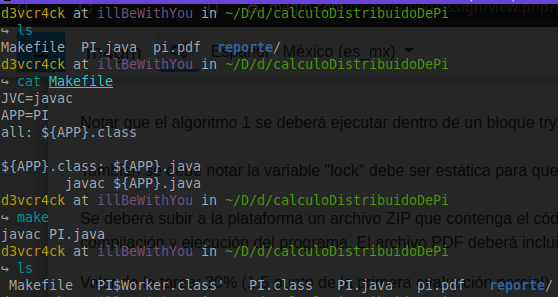
\includegraphics[scale=0.5]{imgs/compilacion.png}
  \\\textit{En esta captura podemos ver la compilación rapida del archivo PI.java gracias al archivo y las tareas que realiza el archivo Makefile y la sencillez de simplemente escribir make en la terminal.}
  \\
  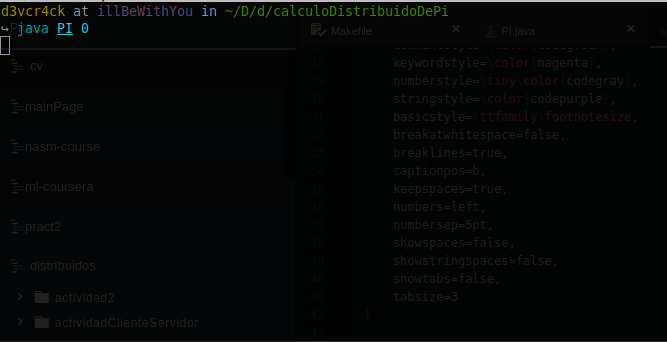
\includegraphics[scale=0.5]{imgs/serverWait.png}
  \\\textit{En esta captura podemos ver que cuando se ejecuta el nodo 0 (Servidor) este se queda esperando a los clientes que se veran involucrados para realizar la serie de Gregory-Leibniz.}
  \\
  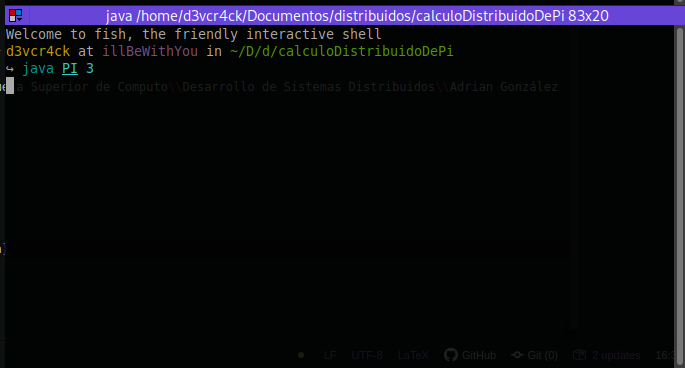
\includegraphics[scale=0.5]{imgs/client-wait.png}
  \\\textit{En esta captura podemos ver que cuando se ejecuta el nodo 3 (Cliente) el cual espera a que este disponible el Servidor (nodo 0), cabe destacar aquí que el server fue parado para mostrar esta funcionalidad.}
  \begin{landscape}
    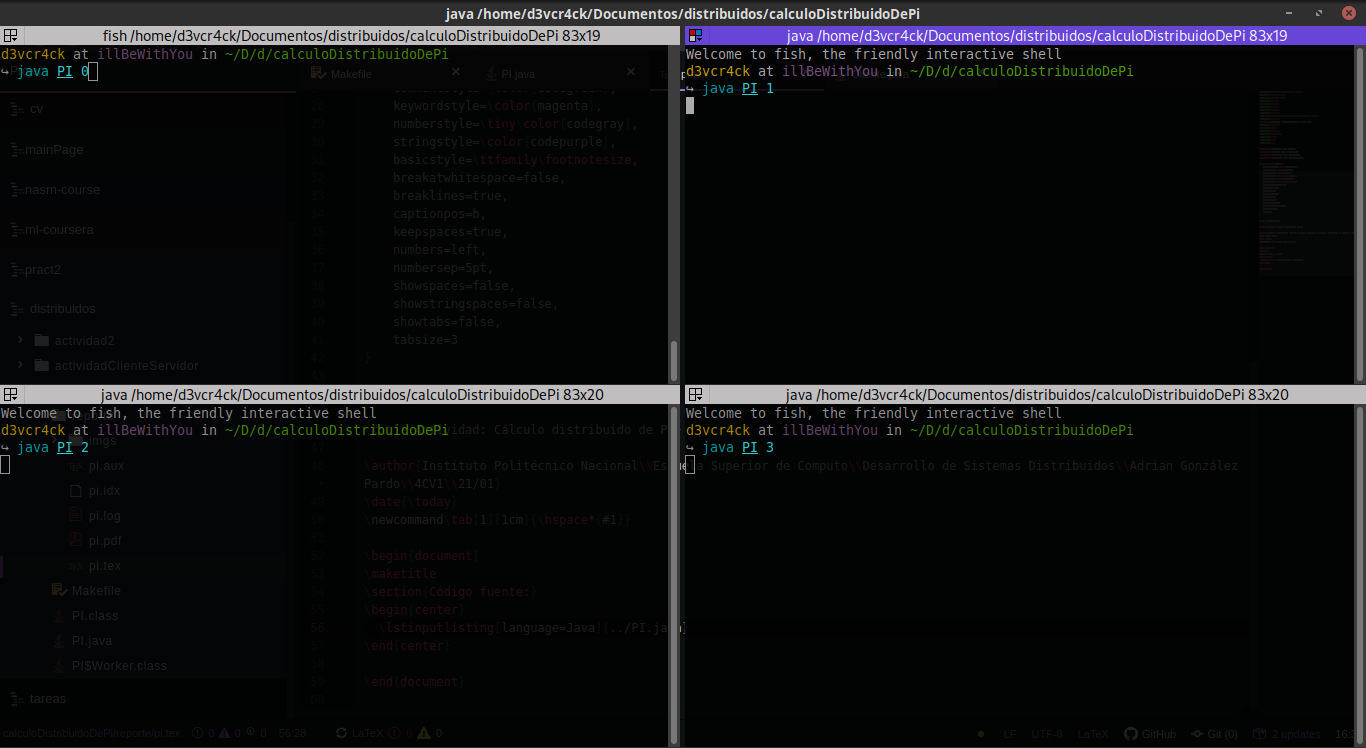
\includegraphics[scale=0.5]{imgs/all-clients-wait-for-server.png}
    \\\textit{En esta captura podemos ver que los nodos 1-3 (Clientes) estan esperando la ejecución del nodo 0 (Servidor) para porder realizar la serie del calculo de $\pi$}\\
  \end{landscape}
  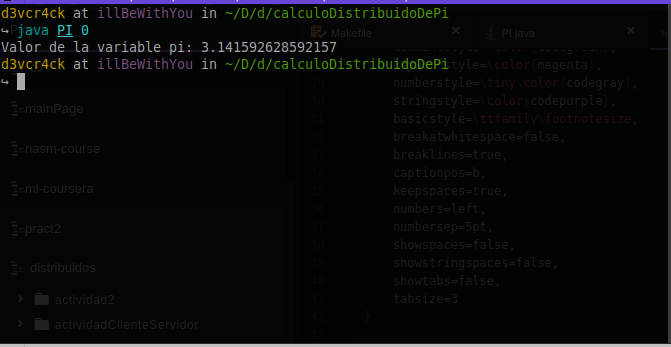
\includegraphics[scale=0.5]{imgs/serverRun-and-exit-when-the-clients-run.png}
  \\\textit{En esta captura podemos ver la ejecución de todos los nodos y de que el nodo 0 muestra el resultado obtenido de la ejecución y unión de los resultados de los nodos 1-3}
\end{center}

\end{document}
